\begin{figure}[t]
\begin{center}
\begin{small}
\begin{sc}

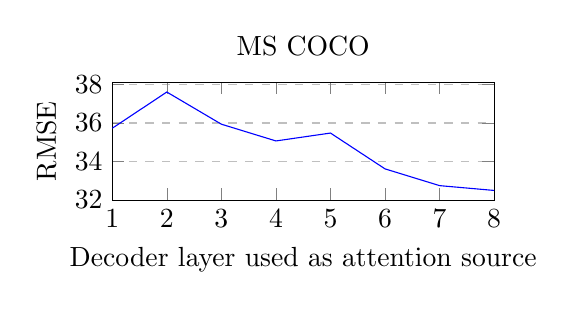
\begin{tikzpicture}
\begin{axis}[
    title={MS COCO},
    xlabel={Decoder layer used as attention source},
    ylabel={RMSE},
    xtick={1,2,3,4,5,6,7,8},
    xmin=1,
    xmax=8,
    ymajorgrids=true,
    grid style=dashed,
    scale only axis,
    height=1.5cm,
    width=.4\textwidth
]
\addplot[color=blue]
    coordinates {
    (1,35.73)(2,37.61)(3,35.94)(4,35.07)(5,35.48)(6,33.62)(7,32.75)(8,32.5)
    };
\end{axis}
\end{tikzpicture}
\end{sc}
\end{small}
\end{center}

\caption{\textbf{RMSE results versus attention map source:} Comparison of attention-based glimpse selection results in regards to decoder layer used as attention map source. The figure shows that the best results can be achieved using the last layer of the decoder. The dataset used is MS COCO. The metric is a root mean square error (RMSE; lower is better). The image resolution is $256\times128$ in an $8\times32^2$ non-retinal glimpse regime.}
\label{fig:attention-layer}
\end{figure}